\documentclass[10pt,a4paper,landscape,twocolumn,twoside]{article}
\usepackage[utf8]{inputenc}
\usepackage[T1]{fontenc}
\usepackage{amsmath}
\usepackage{amssymb}
\usepackage{graphicx}
\graphicspath{ {./Images/} }
\usepackage{xcolor}
\usepackage{wrapfig}
\usepackage{siunitx}
\usepackage[export]{adjustbox}
\usepackage[left=10.00mm, right=10.00mm, top=5.00mm, bottom=15.00mm]{geometry}



\title{Physik 3 \\ [1ex] \large Zusammenfassung}
\author{Sebastian Humbel}


\definecolor{formulablue}{RGB}{219,219,255}
\newcommand{\formula}[1]{\colorbox{formulablue}{#1}}
\newcommand{\unit}[3]{\textit{#1} : #2 [#3]}

\setlength{\parindent}{0pt}







\begin{document}

\section{Optik}
\subsection{Reflexionsgesetz}

\begin{center}
	\begin{minipage}{0.3\textwidth}
		\formula{$\varepsilon' = \varepsilon$} \\
	
		\unitText{$\varepsilon$}{Einfallswinkel}{$rad$} \\
		\unitText{$\varepsilon'$}{Ausfalswinkel}{$rad$}
	\end{minipage}%%% to prevent a space
	\begin{minipage}{0.3\textwidth}
		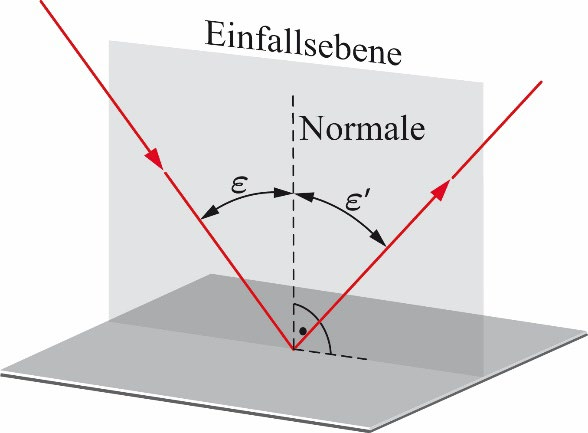
\includegraphics[height=2cm,keepaspectratio=true]{Images/reflexionsgesetz.png}
	\end{minipage}
\end{center}




\subsection{Brechungsgesetz}

Je nach Winkel und Material wird ein Teil reflektiert und ein Teil gebrochen. Ausserdem spielt die Polarisationsrichtung eine Rolle.
\begin{center}
	\begin{minipage}{0.3\textwidth}
		\formula{$\sin(\varepsilon_1) \cdot n_1 = \sin(\varepsilon_2) \cdot n_2 $} 
		\formula{$n = \dfrac{c}{u}$}\\
	
		\unitText{$\varepsilon_1$}{Einfallswinkel}{$rad$} \\
		\unitText{$\varepsilon_1'$}{Ausfalswinkel}{$rad$} \\
		\unitText{$\varepsilon_2$}{Brechungswinkel}{$rad$} \\
		\unitText{$n$}{Brechungsindex}{$1$} \\
		\unitText{$c$}{Vakuum-Lichtgeschwindigkeit (299'792'458)}{$\frac{m}{s^2}$}	
	\end{minipage}%%% to prevent a space
	\begin{minipage}{0.3\textwidth}
		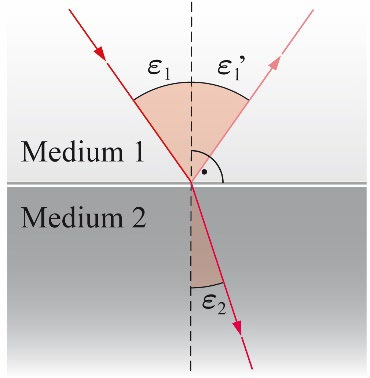
\includegraphics[height=2cm,keepaspectratio=true]{Images/brechungsgesetz.png}
	\end{minipage}
\end{center}




\subsection{Totalreflexion}

\begin{center}
	\begin{minipage}{0.1\textwidth}
		\formula{$\varepsilon_g = \arcsin(\frac{n_1}{n_2}) $}
	\end{minipage}%%% to prevent a space
	\begin{minipage}{0.5\textwidth}
		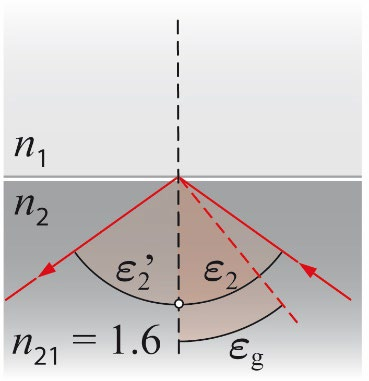
\includegraphics[height=2cm,keepaspectratio=true]{Images/totalreflexion.png}
		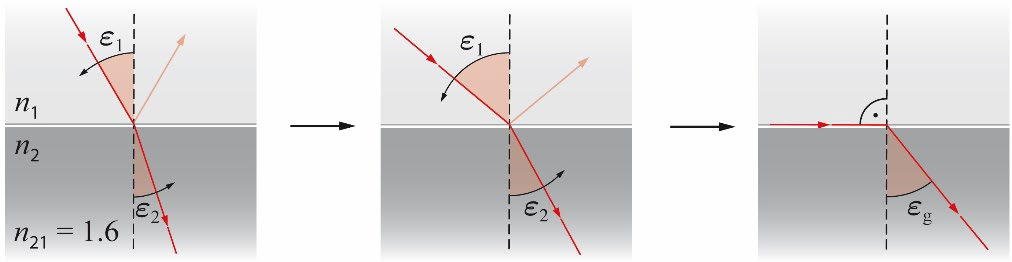
\includegraphics[height=2cm,keepaspectratio=true]{Images/einfallswinkel.png}
	\end{minipage}
\end{center}

\unitText{$\varepsilon_g$}{Grenzwinkel}{$rad$} \\
\unitText{$n_{1,2}$}{Brechungsindex}{$1$}




\subsection{Anwendungen}
\subsubsection{Prisma}

Die \textbf{Minimalablenkung} entsteht wenn der Einfallswinkel gleich dem Ausfallswinkel entspricht.

\begin{center}
	\begin{minipage}{0.3\textwidth}
		\formula{$ \delta_{min} = 2 \arcsin(\frac{n_1}{n_2} \sin(\frac{\varphi}{2})) - \varphi $}
	
		\formula{$ n_2 = \dfrac{\sin\left(\frac{\varphi + \delta_{min}}{2}\right)}{\sin \left(\frac{\varphi}{2}\right) } $}
		
		\formula{$ \delta = \varepsilon_1 + \varepsilon_1' - \varphi $}
	\end{minipage}%%% to prevent a space
	\begin{minipage}{0.3\textwidth}
		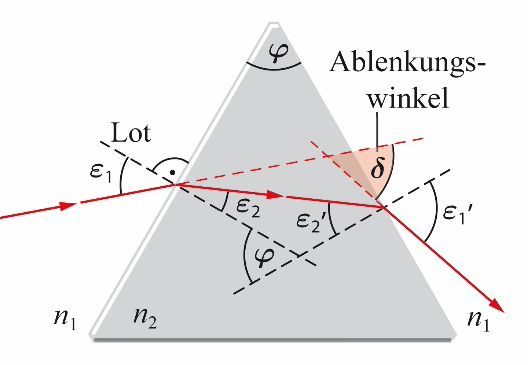
\includegraphics[height=3cm,keepaspectratio=true]{Images/prisma.png}
	\end{minipage}
\end{center}

\unitText{$ n_1 $}{Brechungsindex umgebendes Medium}{$1$} \\
\unitText{$ n_2 $}{Brechungsindex Prisma}{$1$} \\
\unitText{$ \varphi $}{Scheitelwinkel}{$rad$} \\
\unitText{$ \delta $}{Ablenkwinkel}{$rad$} \\

\subsubsection{Lichtwellenleiter}

\begin{center}
	\begin{minipage}{0.3\textwidth}
		Falls $ n_1 > n2 $ :
		\formula{$ \alpha_{1max} = \arcsin\left( \dfrac{n_1 \cos(\arcsin(\frac{n_2}{n_1}))}{n_0} \right)  $}
		\formula{$ n_0 \sin(\alpha_1) = n_1 \sqrt{1 - \cos^2(\alpha_2)} $}
		\formula{$ n_0 \sin(\alpha_1) = n_1 \sqrt{1 - \left( \frac{n_2}{n_1} \right)^2 } $}
		\formula{$ n_0 \sin(\alpha_1) = \sqrt{n_1 ^2 - n_2 ^2} $}
	\end{minipage}%%% to prevent a space
	\begin{minipage}{0.3\textwidth}
		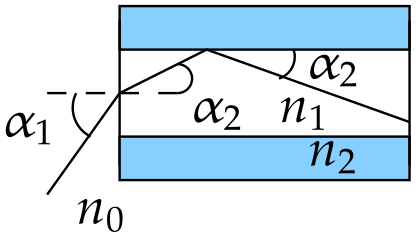
\includegraphics[height=3cm,keepaspectratio=true]{Images/lichtwellenleiter.png}
	\end{minipage}
\end{center}



\subsection{Dispersion}

\begin{center}
	\begin{minipage}{0.25\textwidth}
		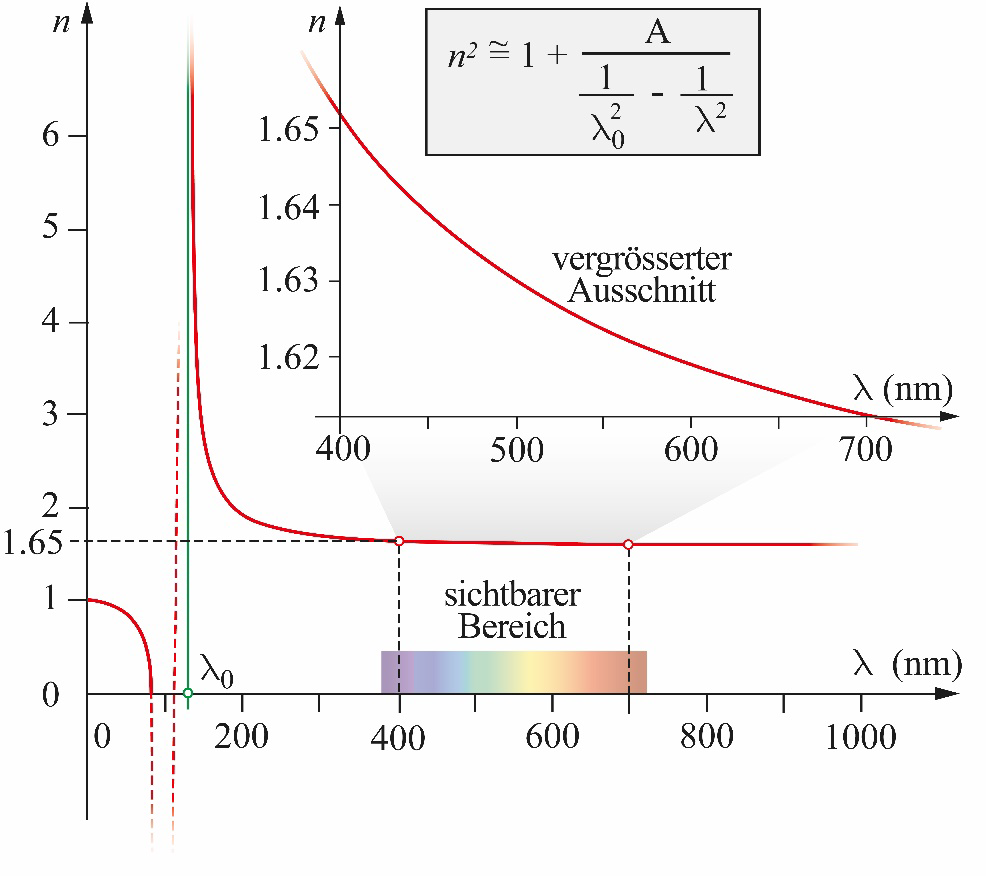
\includegraphics[height=5cm,keepaspectratio=true]{Images/dispersion_graph.png}
	\end{minipage}%%% to prevent a space
	\begin{minipage}{0.3\textwidth}
		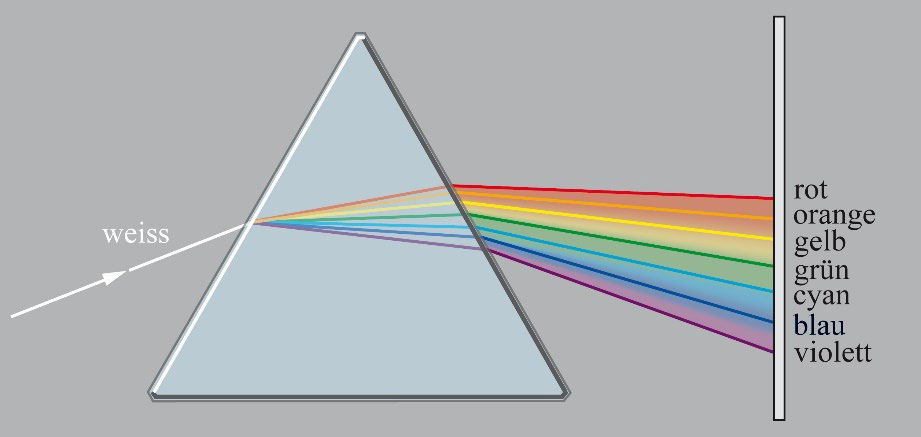
\includegraphics[height=3cm,keepaspectratio=true]{Images/dispersion_prisma.png}
	\end{minipage}
\end{center}


\subsection{Abbildungen}
\subsubsection{Allgemein}
\formula{$ \dfrac{b}{g} = \dfrac{B}{G} = \beta = \dfrac{b - f}{f} $}
\formula{$ \dfrac{1}{f} = \dfrac{1}{g} + \dfrac{1}{b}$} \\
\begin{center}
	\begin{minipage}{0.3\textwidth}
		\unitText{$ b $}{Bildweite}{$ m $} \\
		\unitText{$ g $}{Gegenstandsweite}{$ m $} \\
		\unitText{$ B $}{Bildgrösse}{$ m $}
	\end{minipage}%%% to prevent a space
	\begin{minipage}{0.3\textwidth}
		\unitText{$ G $}{Gegenstansgrösse}{$ m $} \\
		\unitText{$ \beta $}{Abbildungsverhälltniss}{$ 1 $} \\
		\unitText{$ f $}{Brennweite}{$ m $}
	\end{minipage}
\end{center}

\subsubsection{Spiegel}

\textbf{Planspiegel}
\begin{center}
	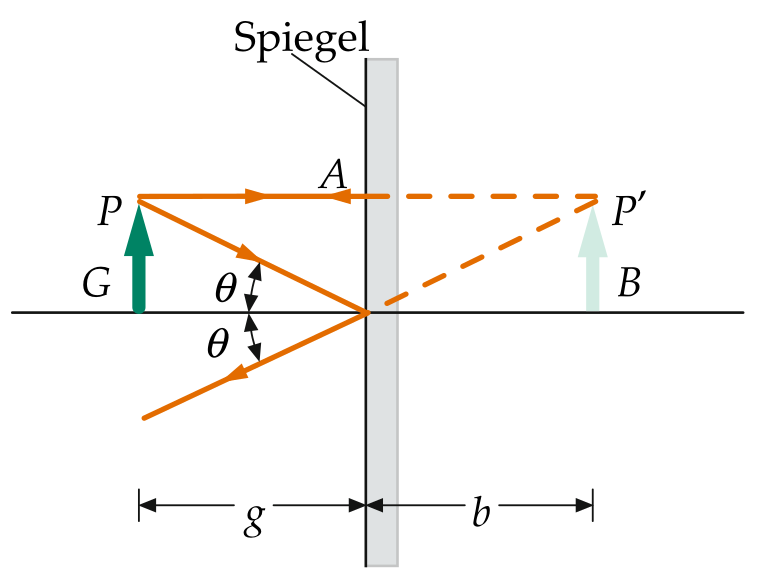
\includegraphics[height=3cm,keepaspectratio=true]{Images/planspiegel.png}
\end{center}


\textbf{Konkavspiegel}

\begin{center}
	\begin{minipage}{0.3\textwidth}
		Für Sphärische Spiegel gilt:
		\formula{$ f = \dfrac{r}{2} $}
	\end{minipage}%%% to prevent a space
	\begin{minipage}{0.3\textwidth}
		\unitText{f}{Brennweite}{$m$} \\
		\unitText{r}{Spiegelradius}{$m$}
	\end{minipage}
\end{center}

\begin{center}
	\begin{minipage}{0.3\textwidth}
		Gegenstand vor dem Brennpunkt. \\
		Erzeugt reeles Bild. \\
		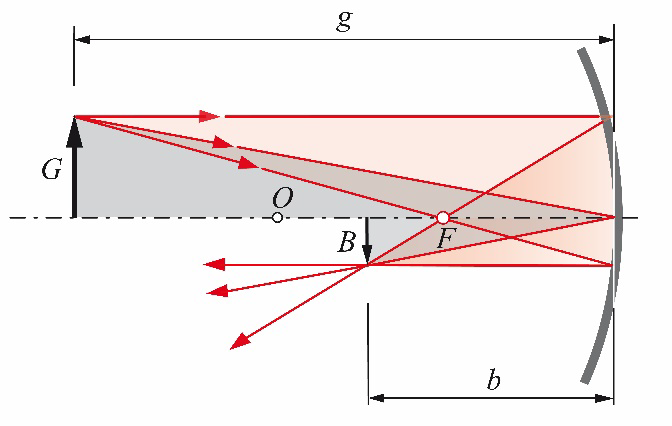
\includegraphics[height=3cm,keepaspectratio=true]{Images/konkavspiegel1.png}
	\end{minipage}%%% to prevent a space
	\begin{minipage}{0.3\textwidth}
		Gegenstand hinter dem Brennpunkt. \\
		Erzeugt virtuelles Bild. \\
		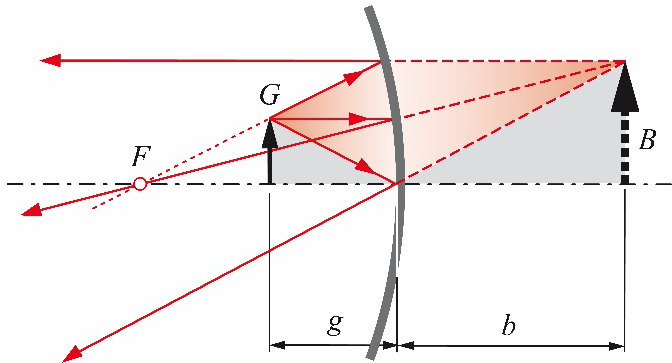
\includegraphics[height=3cm,keepaspectratio=true]{Images/konkavspiegel2.png}
	\end{minipage}
\end{center}


\textbf{Konvexspiegel}
\begin{center}
	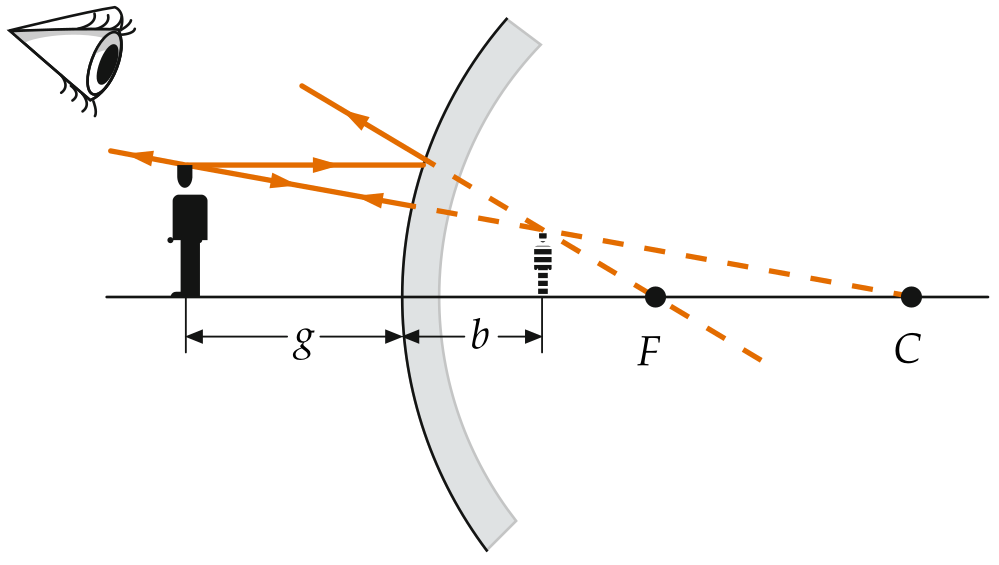
\includegraphics[height=3cm,keepaspectratio=true]{Images/konvexspiegel.png}
\end{center}

\subsubsection{Linsen}

\begin{center}
	\begin{minipage}{0.2\textwidth}
		\formula{$ D = \dfrac{1}{f} $}
		\formula{$ D = \left( \frac{n_2}{n_1} - 1 \right) \left( \frac{1}{r_1} + \frac{1}{r2} \right)  $} \\
		
		\unitText{$ D $}{Brechkraft / Dioptrie}{$1$} \\
		\unitText{$ f $}{Brennweite}{$m$} \\
		\unitText{$ n_{1,2} $}{Brechungsindexe}{$1$} \\
		\unitText{$ r_{1,2} $}{Radien von Linse}{$m$} \\
	\end{minipage}%%% to prevent a space
	\begin{minipage}{0.4\textwidth}
		\begin{itemize}
			\setlength\itemsep{-0.5 em}
			\item Für sammelnde optische Bauelemente ist f > 0.
			\item Für zerstreuende optische Bauelemente f < 0.
			\item Für virtuelle Bilder ist b < 0 und B < 0.
			\item Für virtuelle Gegenstände ist g <	0 und G < 0.
		\end{itemize}
	\end{minipage}
\end{center}

\begin{center}
	\begin{minipage}{0.3\textwidth}
		Bündelnde Linse \\
		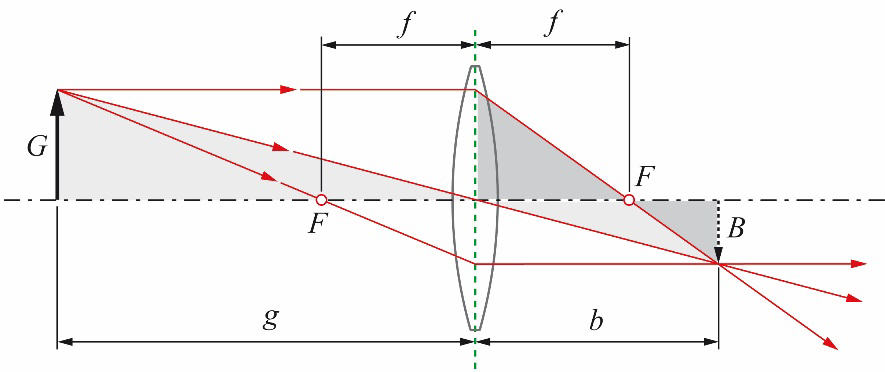
\includegraphics[height=3cm,keepaspectratio=true]{Images/buendelndelinse.png}
	\end{minipage}%%% to prevent a space
	\begin{minipage}{0.3\textwidth}
		Zerstreuende Linse \\
		Brechungsindex negativ! \\
		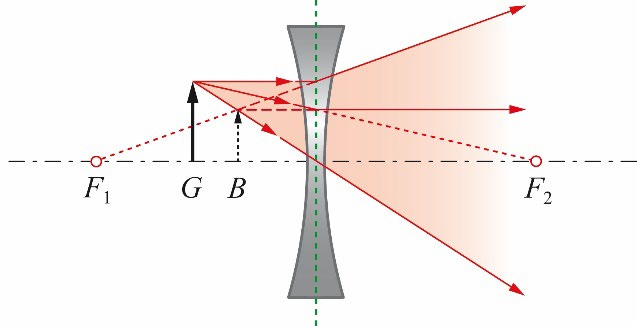
\includegraphics[height=3cm,keepaspectratio=true]{Images/streuendelinse.png}
	\end{minipage}
\end{center}

\subsection{Abbildungssysteme}

\unitText{$ \varepsilon $}{Sehwinkel}{Bogenminute | arcmin | $ 1^\circ = 60\SIUnitSymbolArcminute $} \\
\unitText{$ s $}{deutliche Sehweite (normiert = 25cm)}{m}



\subsubsection{Auflösung, Sehwinkel und Sehweite}

\textbf{Auflösung}: Minimaler Winkelabstand $\varepsilon_min$ zwischen zweier Punkte, welche noch
unterschieden werden können.
\textbf{Sehweite}: Distanz, in der ein Gegenstand noch scharf gesehen werden kann.

Die menschliche Sehschärfe beträgt ca. 1\SIUnitSymbolArcminute.

\begin{center}
	\begin{minipage}{0.2\textwidth}
		\formula{$ S = \dfrac{1}{\varepsilon_{min}} $} \\
		\unitText{$S$}{Sehschärfe}{$\frac{1}{arcmin}$} \\
		\unitText{$\varepsilon$}{Sehwinkel}{$arcmin$} \\
	\end{minipage}%%% to prevent a space
	\begin{minipage}{0.3\textwidth}
		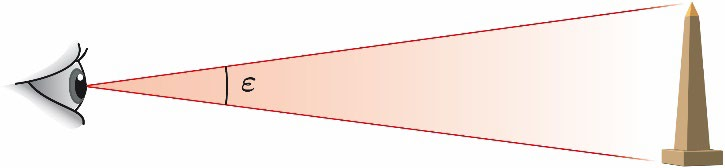
\includegraphics[height=2cm,keepaspectratio=true]{Images/sehwinkel.png}
	\end{minipage}
\end{center}




\subsubsection{Kamera}

\begin{center}
	\begin{minipage}{0.26\textwidth}
		\formula{$ H = \left( \dfrac{d}{f} \right)^2 = q^2 $}
		\formula{$ \dfrac{1}{g} = \dfrac{1}{g_0} \pm \dfrac{u}{q \cdot f^2} $}
		\formula{$ I \sim d^2 $}
		\formula{$ B = \dfrac{f}{g - f} \cdot G $}
		\formula{$ Z = \dfrac{1}{q} = \dfrac{d}{f} $}
		\formula{$ H \sim \dfrac{I}{B^2} \sim \dfrac{d^2}{f^2} $}
	\end{minipage}%%% to prevent a space
	\begin{minipage}{0.3\textwidth}
		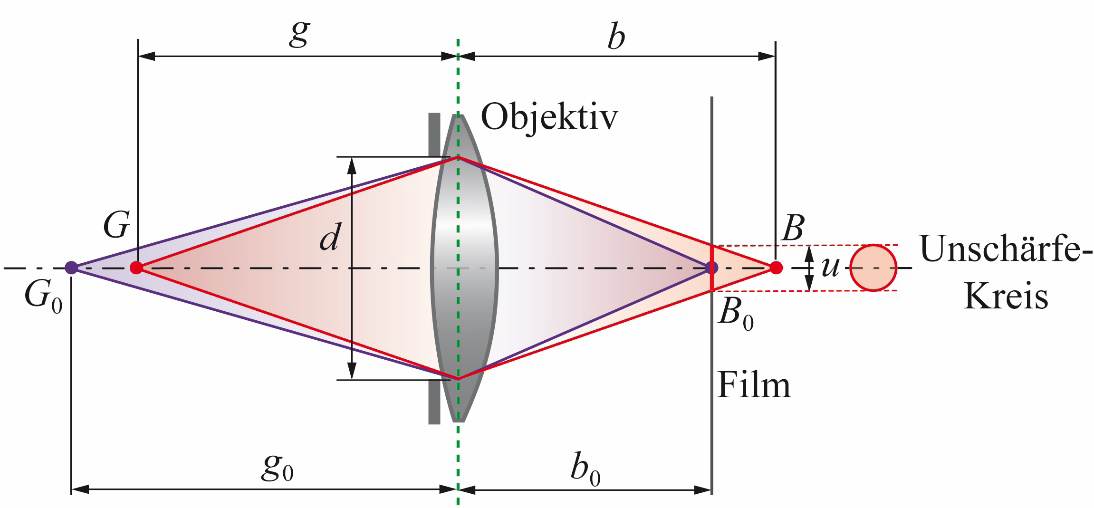
\includegraphics[height=3cm,keepaspectratio=true]{Images/kamera.png}
	\end{minipage}
\end{center}

\begin{center}
	\begin{minipage}{0.3\textwidth}
		\unitText{$ B $}{Bildgrösse}{$ m $} \\
		\unitText{$ G $}{Gegenstandsgrösse}{$ m $} \\
		\unitText{$ H $}{Lichtstärke (Helligkeit)}{$ \frac{W}{m^2} $} \\
		\unitText{$ I $}{Lichtstrom}{$ W $} \\
		\unitText{$ Z $}{Öffnungsverhältnis}{$ 1 $} \\
		\unitText{$ b $}{Bildweite}{$ m $} \\
		\unitText{$ b_0 $}{Filmweite}{$ m $} \\
	\end{minipage}%%% to prevent a space
	\begin{minipage}{0.3\textwidth}
		\unitText{$ d $}{Durchmesser Eintrittspupille}{$ m $} \\
		\unitText{$ f $}{Brennweite}{$ m $} \\
		\unitText{$ g $}{Gegenstandsweite}{$ m $} \\
		\unitText{$ g_0 $}{Schärfentiefenbereich}{$ m $} \\
		\unitText{$ q $}{Blendenzahl}{$ \frac{\sqrt{W}}{m} $} \\
		\unitText{$ u $}{Unschärfenkreis-Durchmesser}{$ m $} \\
	\end{minipage}
\end{center}




\subsubsection{Lupe}

\begin{center}
	\begin{minipage}{0.18\textwidth}
		\formula{$ V = \dfrac{\tan(\varepsilon)}{\tan(\varepsilon_0)} = \dfrac{s}{f} $}
		\formula{$ \tan(\varepsilon) = \dfrac{G}{f} $}
		\formula{$ \tan(\varepsilon_0) = \dfrac{G}{s} $}\\
		
		\unitText{$ V $}{Vergrösserung}{$1$} \\
		\unitText{$ G $}{Gegenstandsgrösse}{$m$} \\
		\unitText{$ \varepsilon $}{Sehwinkel}{$rad$} \\
		\unitText{$ \varepsilon_0 $}{Sehwinkel ohne Lupe}{$rad$} \\
		\unitText{$ s $}{deutliche Sehweite}{$m$} \\
		\unitText{$ f $}{Brennweite}{$m$} \\
	\end{minipage}%%% to prevent a space
	\begin{minipage}{0.3\textwidth}
		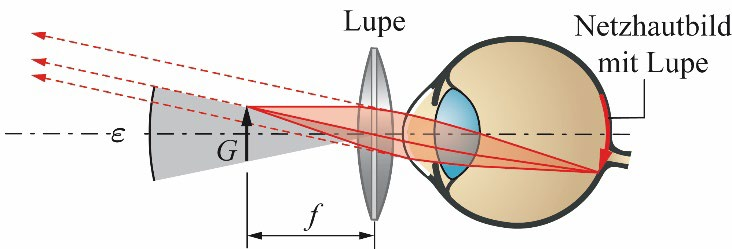
\includegraphics[height=2cm,keepaspectratio=true]{Images/lupe.png}
		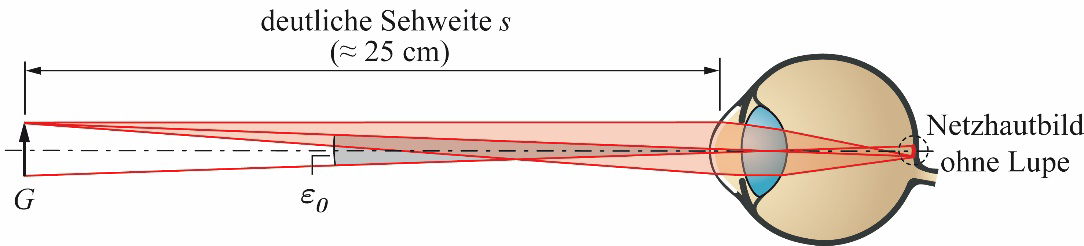
\includegraphics[height=2cm,keepaspectratio=true]{Images/deutliche_sichtweite.png}
	\end{minipage}
\end{center}





\subsubsection{Mikroskop}

\begin{center}
	\begin{minipage}{0.18\textwidth}
		\formula{$ V = \dfrac{\tan(\varepsilon)}{\tan(\varepsilon_0)} $}
		\formula{$ V = \dfrac{\Delta}{f_1} \dfrac{s}{f_2} $}
		\formula{$ V = \dfrac{B}{G} \dfrac{s}{f_2} = \dfrac{b_1}{g_1} \dfrac{s}{f_2} $}
	\end{minipage}%%% to prevent a space
	\begin{minipage}{0.3\textwidth}
		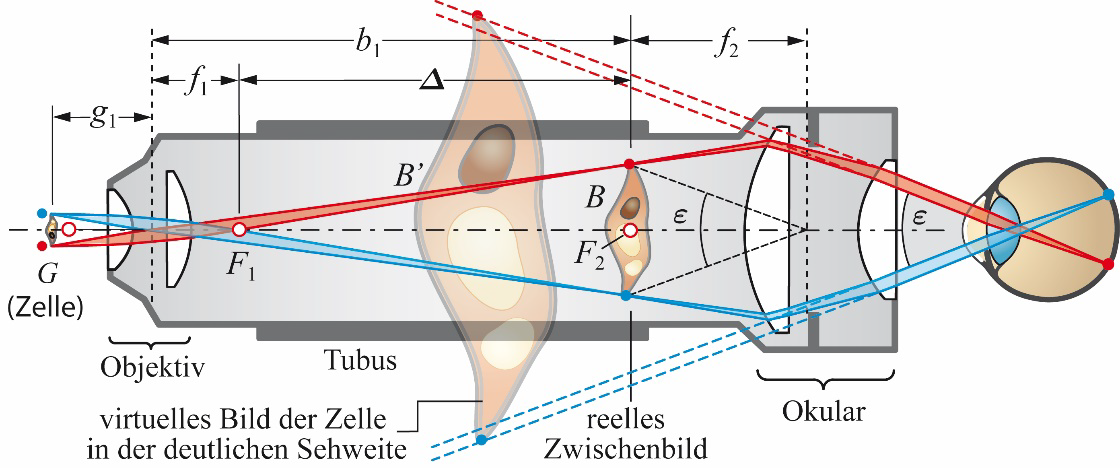
\includegraphics[height=3.5cm,keepaspectratio=true]{Images/mikroskop.png}
	\end{minipage}
\end{center}

\begin{center}
	\begin{minipage}{0.3\textwidth}
		\unitText{$ B $}{Bildgrösse}{$m$} \\
		\unitText{$ G $}{Gegenstandsgrösse}{$m$} \\
		\unitText{$ V $}{Vergrösserung}{$1$} \\
		\unitText{$ \varepsilon $}{Sehwinkel}{$rad$} \\
		\unitText{$ \varepsilon_0 $}{Sehwinkel ohne Mikroskop}{$rad$} \\
	\end{minipage}%%% to prevent a space
	\begin{minipage}{0.3\textwidth}
		\unitText{$ b_1 $}{Bildweite}{$m$} \\
		\unitText{$ f_1 $}{Brennweite Objektiv}{$m$} \\
		\unitText{$ f_2 $}{Brennweite Okular}{$m$} \\
		\unitText{$ s $}{deutliche Sehweite}{$m$} \\
		\unitText{$ \Delta $}{Tubuslänge}{$m$} \\
	\end{minipage}
\end{center}


\subsubsection{Fernrohr}

\begin{center}
	\begin{minipage}{0.2\textwidth}
		\formula{$ V = \dfrac{\tan(\varepsilon)}{\tan(\varepsilon')} = \dfrac{f_1}{f_2}$}
	\end{minipage}%%% to prevent a space
	\begin{minipage}{0.3\textwidth}
		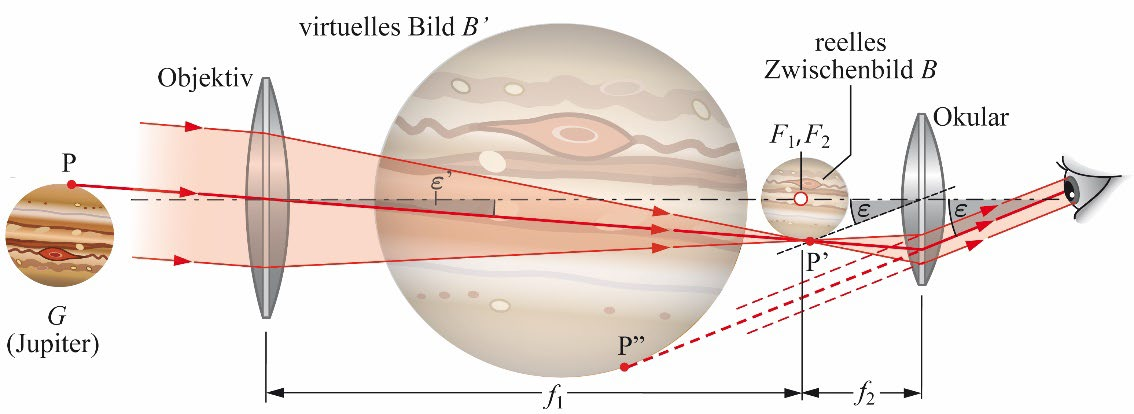
\includegraphics[height=3cm,keepaspectratio=true]{Images/vernrohr.png}
	\end{minipage}
\end{center}

\begin{center}
	\begin{minipage}{0.3\textwidth}
		\unitText{$ V $}{Vergrösserung total}{$1$} \\
		\unitText{$ f_1 $}{Brennweite Objektiv}{$m$} \\
		\unitText{$ f_2 $}{Brennweite Okular}{$m$} \\
	\end{minipage}%%% to prevent a space
	\begin{minipage}{0.3\textwidth}
		\unitText{$ \varepsilon $}{Ausfallswinkel}{$rad$} \\
		\unitText{$ \varepsilon' $}{Einfallswinkel}{$rad$} \\
	\end{minipage}
\end{center}

\subsection{Farbenlehre}

\begin{center}
	\begin{minipage}{0.2\textwidth}
		Subtraktiv \\
		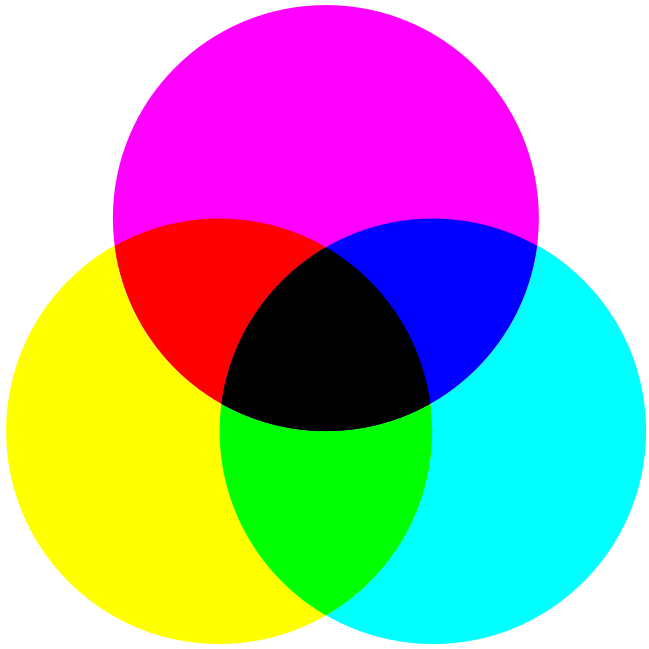
\includegraphics[height=2cm,keepaspectratio=true]{Images/farbenkreise_subtraktiv.png}
	\end{minipage}%%% to prevent a space
	\begin{minipage}{0.2\textwidth}
		Additiv \\
		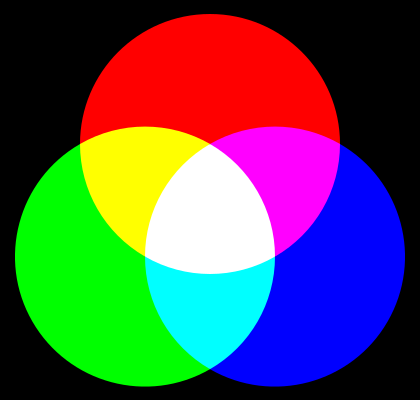
\includegraphics[height=2cm,keepaspectratio=true]{Images/farbenkreise_additiv.png}
	\end{minipage}
\end{center}

\section{Schwingungen}
\subsection{Freie Schwingungen}
\subsubsection{Allgemein}

\formula{$ f = \dfrac{1}{T} $}
\formula{$ \omega = 2 \pi f $}
\formula{$ c = \dfrac{m g}{\Delta l} $}

\begin{center}
	\begin{minipage}{0.3\textwidth}
		Translationsbewegung / Linear \\
		\formula{$ F = m \cdot a $}
	\end{minipage}%%% to prevent a space
	\begin{minipage}{0.3\textwidth}
		Rotationsbewegung / Drehung \\
		\formula{$ M = J \cdot a $}
	\end{minipage}
\end{center}

\begin{center}
	\begin{minipage}{0.3\textwidth}
		\unitText{$f$}{Frequenz}{$ \frac{1}{s} $} \\
		\unitText{$c$}{Federkonstante}{$\frac{N}{m}$} \\
		\unitText{$T$}{Periode}{$ s $} \\
	\end{minipage}%%% to prevent a space
	\begin{minipage}{0.3\textwidth}
		\unitText{$m$}{Masse}{$ kg $} \\
		\unitText{$g$}{Ardanziehung}{$ \frac{m}{s^2} $} \\
		\unitText{$\Delta l$}{Federweg}{$ m $} \\
	\end{minipage}
\end{center}




\subsubsection{Harmonische Schwingung}

\begin{center}
	\begin{minipage}{0.25\textwidth}
		\formula{$ T = \dfrac{2 \pi}{\omega} $}
		\formula{$ y(t) = A \sin( \omega t + \varphi ) $}
		\formula{$ v(t) = \dot{y} = A \omega_0 \cos(\omega_0 t) $}
		\formula{$ a(t) = \ddot{y} = - A \omega_0 ^2 \sin(\omega_0 t) $} \\
		
		\unitText{$A$}{Amplitude}{$1$} \\
		\unitText{$\omega$}{Kreisfrequenz}{$\frac{1}{s}$} \\
		\unitText{$t$}{Zeit}{$s$} \\
		\unitText{$\varphi$}{Phasenverschiebung}{$rad$}
	\end{minipage}%%% to prevent a space
	\begin{minipage}{0.3\textwidth}
		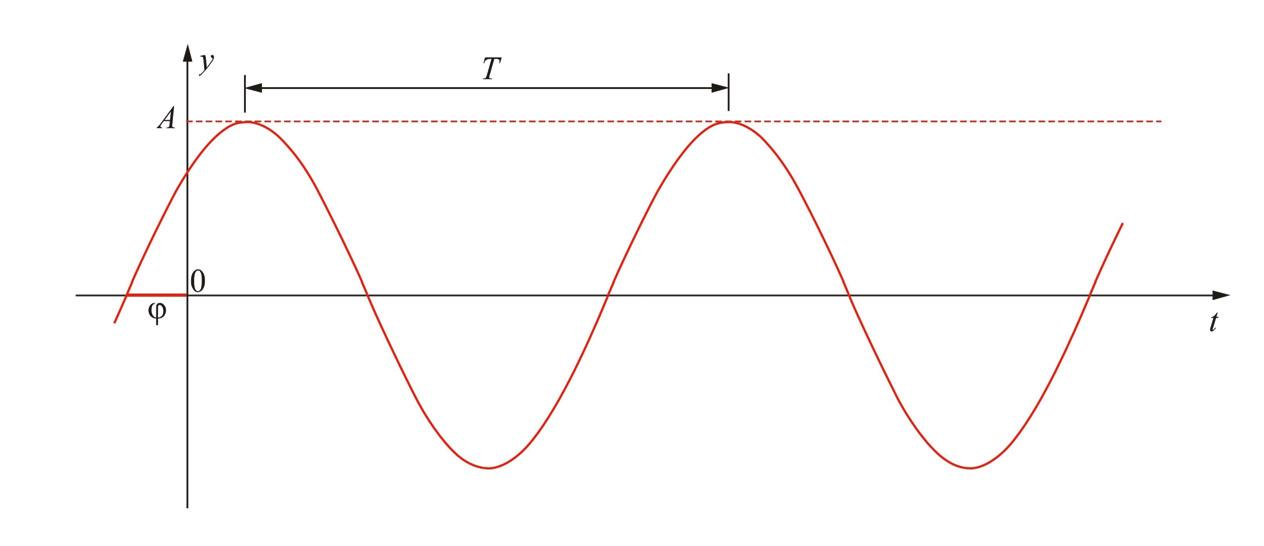
\includegraphics[height=3cm,keepaspectratio=true]{Images/harmonische_schwingung.png}
	\end{minipage}
\end{center}



\subsubsection{Federpendel}

\begin{center}
	\begin{minipage}{0.2\textwidth}
		\formula{$ F_1 = - F_{10} - c_1 \cdot y $}
		\formula{$ F_2 = F_{20} - c_2 \cdot y = F_0 - c \cdot y $}
		\formula{$ F_{RES} = -c \cdot y = F_1 + F_2 $}
		\formula{$ T = 2 \pi \sqrt{\dfrac{m}{c}} = \dfrac{2 \pi}{\omega_0} $}
		\formula{$ T = 2 \pi \sqrt{\dfrac{m + \dfrac{m_F}{3}}{c}} $)}
	\end{minipage}%%% to prevent a space
	\begin{minipage}{0.3\textwidth}
		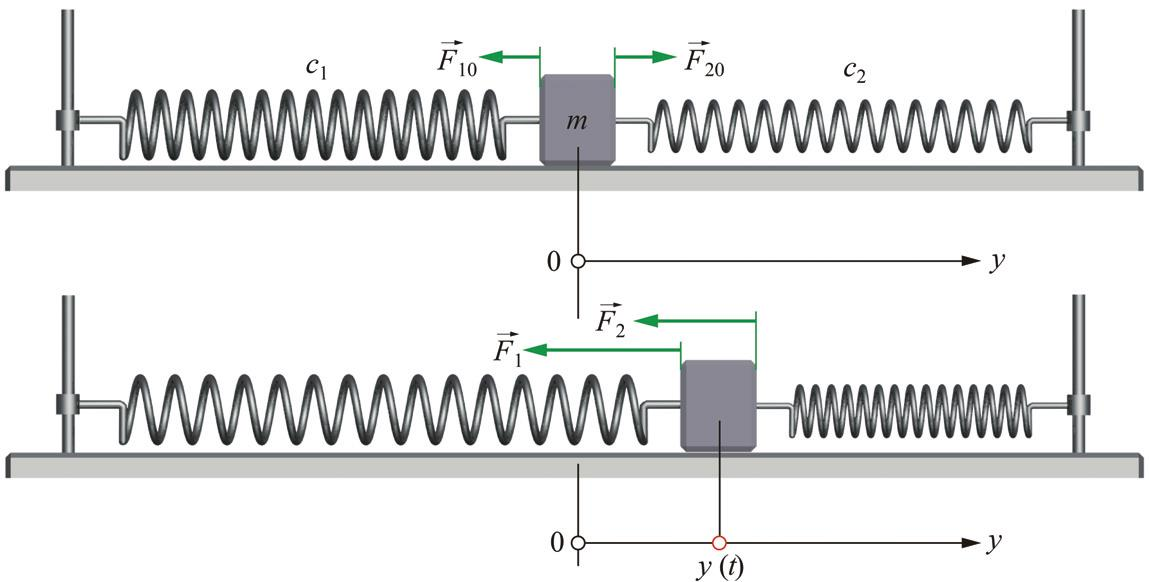
\includegraphics[height=4cm,keepaspectratio=true]{Images/federpendel.png}
	\end{minipage}
\end{center}

\formula{$ a(t) = - \left( \dfrac{c}{m} \right) y $}
\formula{$ y(t) = A \sin(\omega_0 t + \varphi) $}
\formula{$ \omega_0 = \sqrt{\dfrac{c}{m}} $}
\formula{$ m \ddot{y} + c y = 0 $}

\begin{center}
	\begin{minipage}{0.3\textwidth}
		\unitText{$F_x$}{Kraft}{$N$} \\
		\unitText{$T$}{Periode}{$s$} \\
		\unitText{$a$}{Beschleunigung}{$\frac{m}{s^2}$} \\
		\unitText{$c$}{Federkonstante}{$\frac{N}{m}$} \\
		\unitText{$m$}{Bewegte Masse}{$kg$}
	\end{minipage}%%% to prevent a space
	\begin{minipage}{0.3\textwidth}
		\unitText{$m_F$}{Federmasse}{$kg$} \\
		\unitText{$t$}{Zeit}{$sekunden$} \\
		\unitText{$y$}{Auslenkung}{$m$} \\
		\unitText{$\omega$}{Kreisfrequenz}{$\frac{1}{s}$} \\
		\unitText{$\varphi$}{Nullphasenwinkel}{$rad$}
	\end{minipage}
\end{center}





\subsubsection{Drehpendel (Torsionspendel)}

\begin{center}
	\begin{minipage}{0.3\textwidth}
		\formula{$M = -c \varphi(t)$}
		\formula{$J = J_s + 2 m l^2$}
		\formula{$J \cdot \ddot{y} + c \cdot \varphi = 0$}
		\formula{$\omega = \sqrt{\dfrac{c}{J}}$}
		\formula{$T = 2 \pi \sqrt{\dfrac{J}{c}}$}
	\end{minipage}%%% to prevent a space
	\begin{minipage}{0.3\textwidth}
		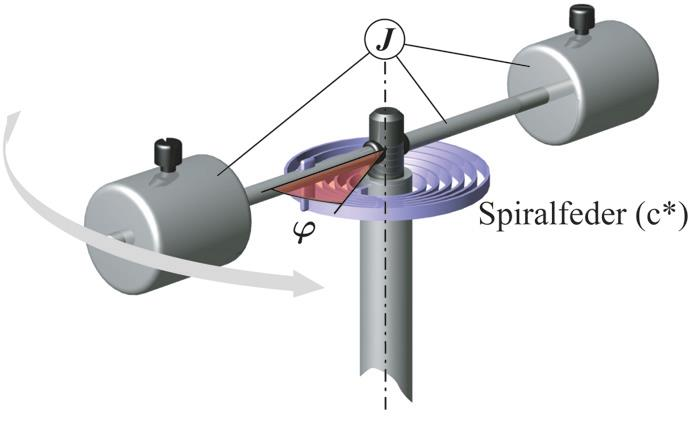
\includegraphics[height=3cm,keepaspectratio=true]{Images/drehpendel.png}
	\end{minipage}
\end{center}
\begin{center}
	\begin{minipage}{0.3\textwidth}
		\unitText{$J$}{Massenträgheitmoment}{$\frac{kg}{m^2}$} \\
		\unitText{$M$}{Drehmoment}{$N m$} \\
		\unitText{$T$}{Periode}{$s$}
	\end{minipage}%%% to prevent a space
	\begin{minipage}{0.3\textwidth}
		\unitText{$c$}{Federkonstant}{$\frac{N}{m}$} \\
		\unitText{$y$}{Auslemkung}{$m$} \\
		\unitText{$\omega$}{Kreisfrequenz}{$\frac{1}{s}$} \\
		\unitText{$\varphi$}{Nullphasenwinkel}{$rad$}	
	\end{minipage}
\end{center}






\subsubsection{Schwerependel Mathematisch}
\begin{center}
	\begin{minipage}{0.3\textwidth}
		\formula{$M = l \cdot m \cdot g \cdot \sin(\varphi)$}
		\formula{$J = J_s + m \cdot l^2 = 0 + m \cdot l^2$}
		\formula{$T = 2 \pi \sqrt{\dfrac{l}{g}}$}
		\formula{$\omega_0 = \sqrt{\dfrac{g}{l}}$}
		\formula{$l \ddot{y} + g \sin(\varphi) = 0$}
		\formula{$l \ddot{y} + g \varphi = 0$}
	\end{minipage}%%% to prevent a space
	\begin{minipage}{0.3\textwidth}
		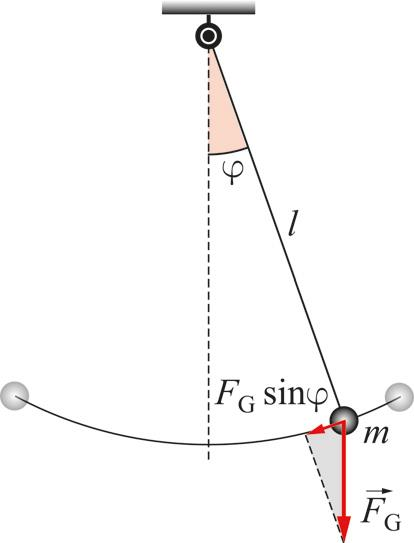
\includegraphics[height=4cm,keepaspectratio=true]{Images/schwerependel_mathematisch.png}
	\end{minipage}
\end{center}

\begin{center}
	\begin{minipage}{0.3\textwidth}
		\unitText{$J$}{Massenträgheitmoment}{$\frac{kg}{m^2}$} \\
		\unitText{$M$}{Drehmoment}{$N m$} \\
		\unitText{$T$}{Periode}{$s$} \\
		\unitText{$g$}{Erdbeschleunigung}{$\frac{m}{s^2}$}
	\end{minipage}%%% to prevent a space
	\begin{minipage}{0.3\textwidth}
		\unitText{$l$}{Pendellänge}{$m$} \\
		\unitText{$y$}{Auslemkung}{$m$} \\
		\unitText{$\omega$}{Kreisfrequenz}{$\frac{1}{s}$} \\
		\unitText{$\varphi$}{Winkel}{$rad$}
	\end{minipage}
\end{center}




\subsubsection{Schwerependel Physikalisch}
\begin{center}
	\begin{minipage}{0.3\textwidth}
		\formula{$T = 2 \pi \sqrt{\dfrac{J_A}{m \cdot g \cdot a}} =
			2 \pi \sqrt{\dfrac{J_S + m a^2}{m \cdot g \cdot a}} $}
		\formula{$\omega_0 = \sqrt{\dfrac{m \cdot g \cdot a}{J_A}}$}
		\formula{$l^* = \dfrac{J_A}{m a}$}
		\formula{$J_A \ddot{\varphi} = m \cdot g \cdot a \cdot \sin(\varphi) = 0 $}
		\formula{$J_A = J_S + m a^2$}
		\formula{$\omega_{max} = \sqrt{\dfrac{g}{2} \sqrt{\dfrac{m}{J_S}}}$}
		
	\end{minipage}%%% to prevent a space
	\begin{minipage}{0.3\textwidth}
		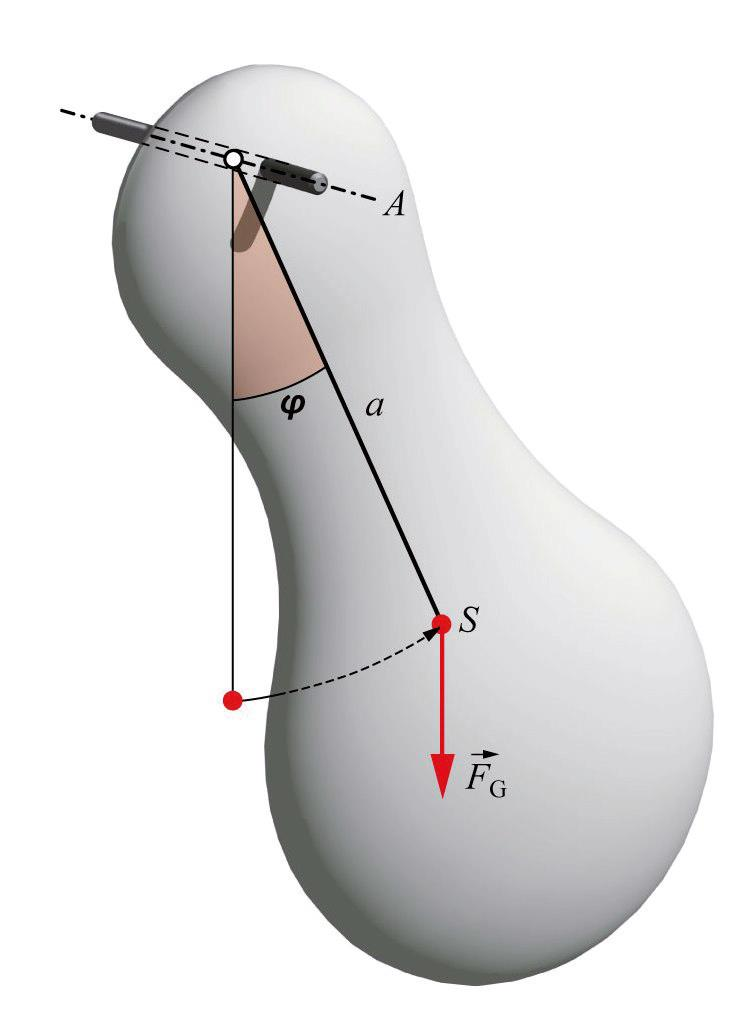
\includegraphics[height=4cm,keepaspectratio=true]{Images/schwerependel_physikalisch.png}
	\end{minipage}
\end{center}

\begin{center}
	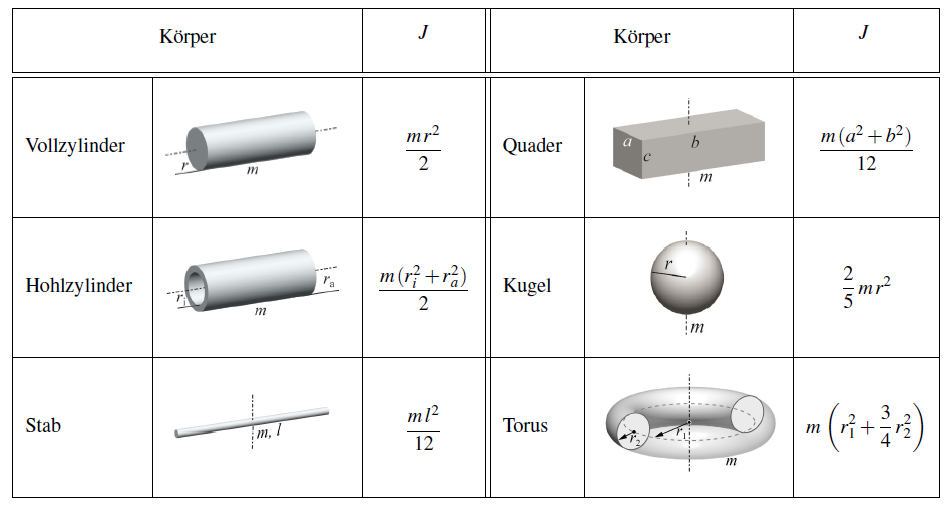
\includegraphics[height=7cm,keepaspectratio=true]{Images/traegheitsmomente.png}
\end{center}
\begin{center}
	\begin{minipage}{0.3\textwidth}
		\unitText{$J_A$}{Massenträgheit bez. A-Achse}{$kg \cdot m^2$} \\
		\unitText{$J_S$}{Massenträgheit bez. Achse $\parallel$ a}{$kg \cdot m^2$} \\
		\unitText{$T$}{Periode}{$s$} \\
		\unitText{$a$}{Abstand zum Schwerpunkt S}{$m$} \\
	\end{minipage}%%% to prevent a space
	\begin{minipage}{0.3\textwidth}
		\unitText{$g$}{Erdbeschleunigung}{$\frac{m}{s^2}$} \\
		\unitText{$m$}{Masse}{$kg$} \\
		\unitText{$l^*$}{Reduzierte Pendellänge}{$m$} \\
		\unitText{$\omega_0$}{Kreisfrequenz}{$\frac{1}{s}$} \\
	\end{minipage}
\end{center}


\subsubsection{Perkussionszentrum}
\begin{center}
	\begin{minipage}{0.3\textwidth}
		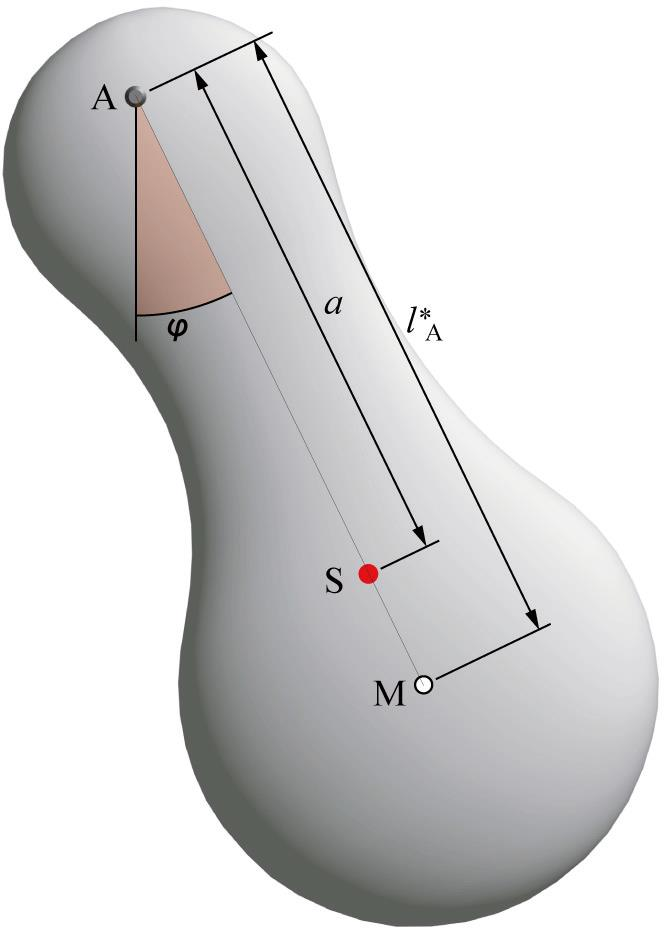
\includegraphics[height=4cm,keepaspectratio=true]{Images/schwerependel_perkussionszentrum.png}
	\end{minipage}%%% to prevent a space
	\begin{minipage}{0.3\textwidth}
		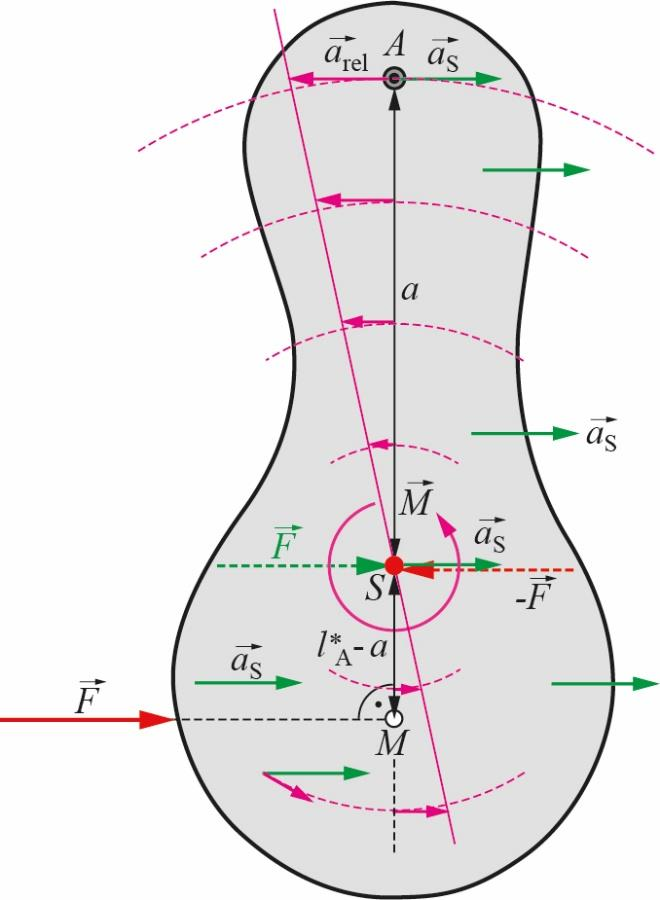
\includegraphics[height=4cm,keepaspectratio=true]{Images/perkussionszentrum.png}
	\end{minipage}
\end{center}




\subsubsection{Energie}
\begin{center}
	\begin{minipage}{0.2\textwidth}
		\formula{$E_{ges} = \frac{1}{2} c A^2 = E_{pot} + E_{kin}$} \\
		\formula{$E_{pot} = \frac{1}{2} c A^2 \cos^2(\omega t + \varphi)$} \\
		\formula{$E_{kin} = \frac{1}{2} c A^2 \sin^2(\omega t + \varphi)$} \\
		
		\unitText{$E_{xyz}$}{Energie}{$J$} \\
		\unitText{$A$}{Amplitude}{$m$} \\
		\unitText{$c$}{Federkonstante}{$\frac{N}{m}$} \\
		\unitText{$t$}{Zeit}{$s$} \\
		\unitText{$\omega$}{Kreisfrequenz}{$\frac{1}{s}$}
	\end{minipage}%%% to prevent a space
	\begin{minipage}{0.3\textwidth}
		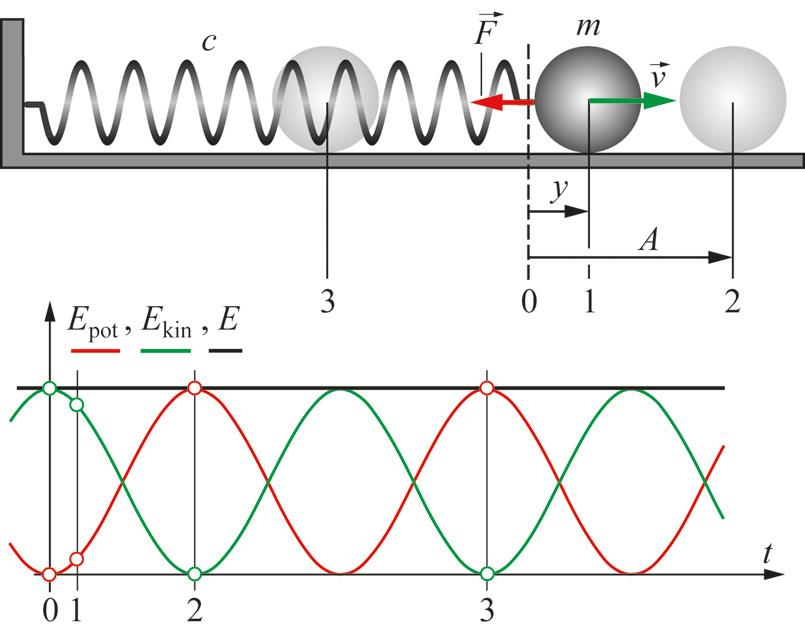
\includegraphics[height=4.5cm,keepaspectratio=true]{Images/schwingung_energie.png}
	\end{minipage}
\end{center}




\subsubsection{Gedämpfte Schwingung}
\begin{center}
	\begin{minipage}{0.2\textwidth}
		\formula{$F_G = m g$}
		\formula{$F_F = -c y$}
		\formula{$F_D = -b \dot{y}$}
		\formula{$m \ddot{y} + b \dot{y} + c y = 0$}
		\formula{$y = A e^{- \delta t} \sin(\omega_d t + \varphi_0)$}
		\formula{$\delta = \dfrac{b}{2 m}$}
		\formula{$\varLambda = \delta T$}
		\formula{$\varLambda = \ln \left(  \frac{A_n}{A_{n+1}} \right) $}
		\formula{$D = \dfrac{\delta}{\omega_0}$}
		\formula{$\dfrac{A_n}{A_{n+1}} = e^{\delta T}$}
		\formula{$m \ddot{y} = F_{Res} = F_F - F_G + F_D$}
	\end{minipage}%%% to prevent a space
	\begin{minipage}{0.3\textwidth}
		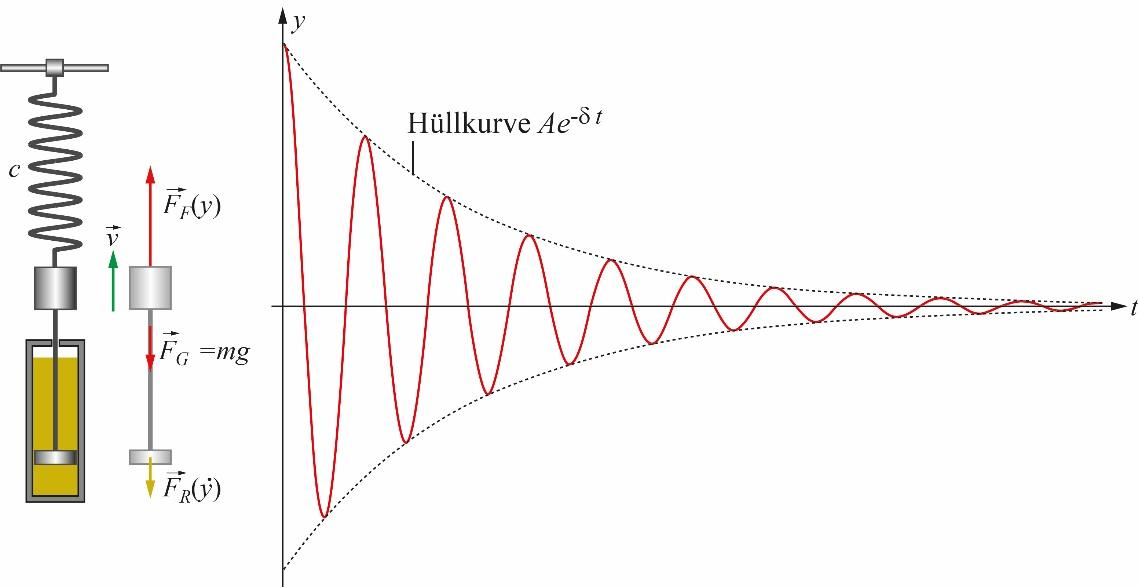
\includegraphics[height=4.5cm,keepaspectratio=true]{Images/gedaempfte_schwingung.png}
	\end{minipage}
\end{center}
\begin{center}
	\begin{minipage}{0.3\textwidth}
		\unitText{$A$}{Amplitude}{$m$} \\
		\unitText{$D$}{Dämpfungsgrad}{$1$} \\
		\unitText{$F_G$}{Gewichtskraft}{$N$} \\
		\unitText{$F_F$}{Federkraft}{$N$} \\
		\unitText{$F_D$}{Dämpfungskraft}{$N$} \\
		\unitText{$T$}{Periode}{$s$} \\
		\unitText{$b$}{Dämpfungskonstante}{$1$}
	\end{minipage}%%% to prevent a space
	\begin{minipage}{0.3\textwidth}
		\unitText{$c$}{Federkonstante}{$\frac{N}{m}$} \\
		\unitText{$m$}{Masse}{$kg$} \\
		\unitText{$y$}{Auslenkung}{$m$} \\
		\unitText{$\delta$}{Abklingkonstante}{$1$} \\
		\unitText{$\varphi$}{Nullphasenwinkel}{$rad$} \\
		\unitText{$\omega$}{Kreisfrequenz}{$\frac{1}{s}$} \\
		\unitText{$\varLambda$}{log. Dekrement}{$1$}
	\end{minipage}
\end{center}

\subsection{Fremderregte Schwingung}
\textbf{Formelsammlung Sourlier 22.1.6 p.574}
\begin{center}
	\begin{minipage}{0.28\textwidth}
		\unitText{$\omega$}{Kreisfrequenz der Störung}{$\frac{rad}{s}$} \\
		\unitText{$\omega_0$}{Kreisf. ungedämpfter Schwingung}{$\frac{rad}{s}$} \\
		\unitText{$\omega_d$}{Kreisf. gedämpfter Schwingung}{$\frac{rad}{s}$} \\
		\unitText{$\omega_r$}{Resonanzkreisfrequenz}{$\frac{rad}{s}$} \\
		\unitText{$\delta$}{Abklingkonstante}{$\frac{1}{s}$}
	\end{minipage}
	\begin{minipage}{0.2\textwidth}
		\unitText{$\eta$}{dimensionslose Frequenz}{$1$} \\
		\unitText{$\varphi$}{Phase}{$rad$} \\
		\unitText{$A$}{Amplitude}{$m$} \\
		\unitText{$A_r$}{Resonanzamplitude}{$m$} \\
		\unitText{$D$}{Dämpfungsgrad}{$1$} \\
		\unitText{$V$}{Vergrösserungsfunktion}{$?$}
	\end{minipage}
\end{center}
\subsubsection{Krafterregung und Federkrafterregung}
\begin{center}
	\begin{minipage}{0.3\textwidth}
		\formula{$m \ddot{y} + b \dot{y} + c y = c u_0 \sin(\omega t)$}
		\formula{$\omega_r = \omega_0 \sqrt{1 - 2 D^2}$}
		\formula{$A = \dfrac{c u_0}{m \sqrt{(\omega^2_0 - \omega^2)^2 + (2 D \omega_0 \omega)^2}}$}
		\formula{$\omega_d = \sqrt{\omega^2_0 - \delta^2}$}
		\formula{$\varphi = \arctan \dfrac{2 D \omega_0 \omega}{\omega^2_0 - \omega^2}$}
		\formula{$A_r = \dfrac{u_0}{2 D \sqrt{1 - D^2}}$}
		\formula{$V = \dfrac{1}{\sqrt{(1 - \eta^2)^2 + (2 D \eta)^2}}$}
		\formula{$D = \dfrac{\delta}{\omega_0}$}
	\end{minipage}%%% to prevent a space
	\begin{minipage}{0.2\textwidth}
		\begin{center}
			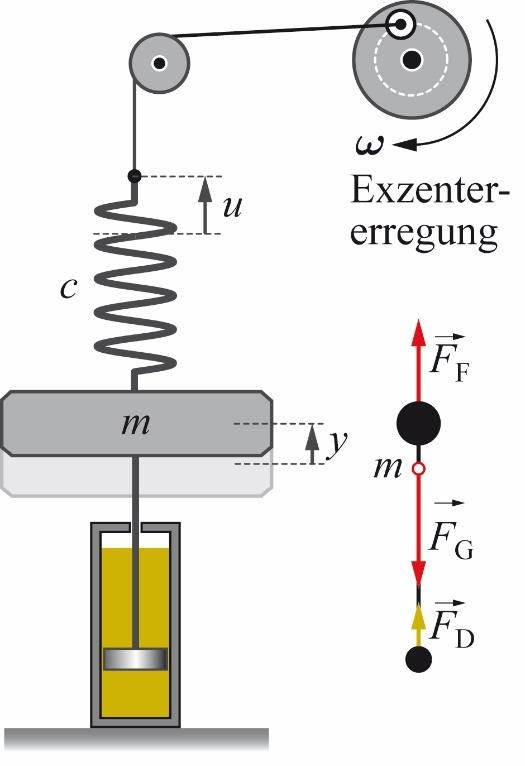
\includegraphics[height=4cm,keepaspectratio=true]{Images/krafterregung_a.png}
			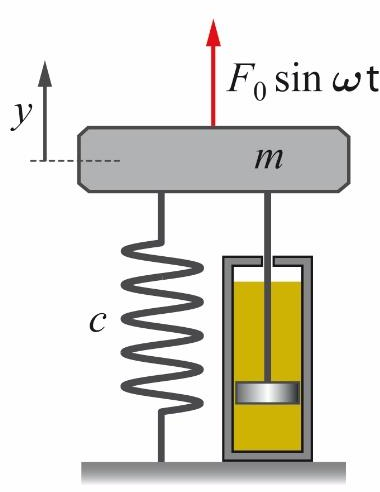
\includegraphics[height=3cm,keepaspectratio=true]{Images/krafterregung_b.png}
		\end{center}
	\end{minipage}
\end{center}

\subsubsection{Indirekte Federkrafterregung}
\formula{$m \ddot{y} + b \dot{y} + c y = c_2 u_0 \sin(\omega t)$}
\formula{$A = \dfrac{c_2}{c} \dfrac{c u_0}{m \sqrt{(\omega^2_0 - \omega^2)^2 + (2 D \omega_0 \omega)^2}}$}
\formula{$\varphi = \arctan \dfrac{2 D \omega_0 \omega}{\omega^2_0 - \omega^2}$}
\formula{$\omega_r = \omega_0 \sqrt{1 - 2 D^2}$}
\formula{$A_r = \dfrac{u_0}{2 D \sqrt{1 - D^2}}$}
\formula{$V = \dfrac{c_2}{c} \dfrac{1}{\sqrt{(1 - \eta^2)^2 + (2 D \eta)^2}}$}






\subsubsection{Dämpferregung}
\begin{center}
	\begin{minipage}{0.4\textwidth}
		\formula{$m \ddot{y} + b \dot{y} + c y = b \omega u_0 \sin(\omega t + \dfrac{\pi}{2})$}
		\formula{$V = \dfrac{2 D \eta}{\sqrt{(1 - \eta^2)^2 + (2 D \eta)^2}}$}
		\formula{$A = \dfrac{b \omega u_0}{m \sqrt{(\omega^2_0 - \omega^2)^2 + (2 D \omega_0 \omega)^2}}$}
		\formula{$\varphi = \arctan \dfrac{2 D \omega_0 \omega}{\omega^2_0 - \omega^2} - \dfrac{\pi}{2}$}
		\formula{$\omega_r = \omega_0$}
		\formula{$A_r = u_0$}
		\formula{$V = \dfrac{2 D \eta}{\sqrt{(1 - \eta^2)^2 + (2 D \eta)^2}}$}
	\end{minipage}%%% to prevent a space
	\begin{minipage}{0.1\textwidth}
		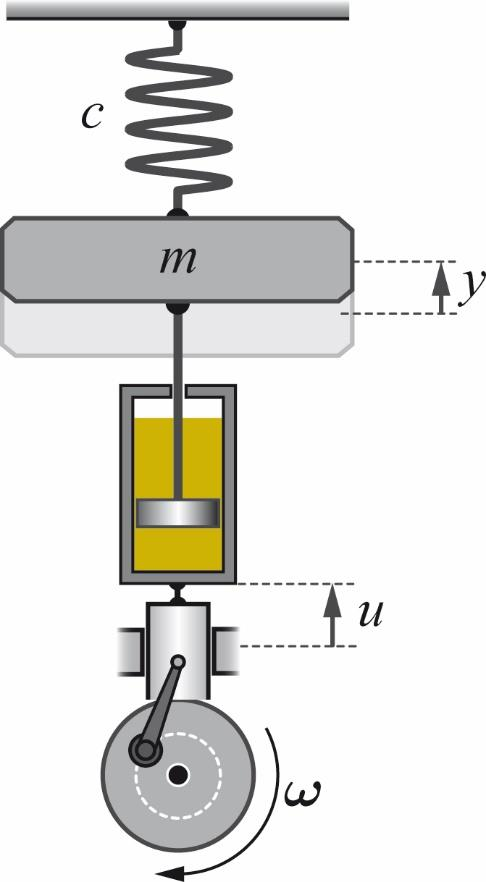
\includegraphics[height=3cm,center,keepaspectratio=true]{Images/daempferregung.png}
	\end{minipage}
\end{center}


\subsubsection{Stützerregung}
\begin{center}
	\begin{minipage}{0.4\textwidth}
		\formula{$m \ddot{y} + b \dot{y} + c y = c u_0 \sin(\omega t) + b \omega u_0 \cos(\omega t)$}
		\formula{$m \ddot{q} + b \dot{q} + c q = m \omega^2 u_0 \sin(\omega t)$}
		\formula{$A = \dfrac{\omega^2 u_0}{\sqrt{(\omega^2_0 - \omega^2)^2 + (2 D \omega_0 \omega)^2}}$}
		\formula{$\varphi = \arctan \left(  \dfrac{2 D \omega_0 \omega}{\omega^2_0 - \omega^2} \right) - \pi$}
		\formula{$\omega_r = \dfrac{\omega_0}{\sqrt{1 - 2 D^2}}$}
		\formula{$A_r = \dfrac{u_0}{2 D \sqrt{1 - D^2}}$}
		\formula{$V = \dfrac{\eta^2}{\sqrt{(1 - \eta^2)^2 + (2 D \eta)^2}}$}
	\end{minipage}%%% to prevent a space
	\begin{minipage}{0.1\textwidth}
	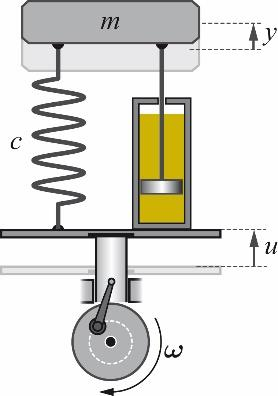
\includegraphics[height=3cm,center,keepaspectratio=true]{Images/stuezerregung.png}
	\end{minipage}
\end{center}

\pagebreak

\subsubsection{Unwuchterregung}
\begin{center}
	\begin{minipage}{0.25\textwidth}
		\formula{$m \ddot{y} + b \dot{y} + c y = m_R e \omega \sin(\omega t)$}
		\formula{$A = \dfrac{m_R e \omega^2}{\sqrt{(\omega^2_0 - \omega^2)^2 + (2 D \omega_0 \omega)^2}}$}
		\formula{$\varphi = \arctan \dfrac{2 D \omega_0 \omega}{\omega^2_0 - \omega^2}$}
		\formula{$\omega_r = \dfrac{\omega_0}{\sqrt{1 - 2 D^2}}$}
		\formula{$A_r = \dfrac{m_R}{m} = \dfrac{e}{2 D \sqrt{1 - D^2}}$}
		\formula{$\dfrac{F_{B0}}{F_0} = \sqrt{\dfrac{1 + 4 D^2 \eta^2}{(1 - \eta^2)^2 + 4 D^2 \eta^2}}$}
	\end{minipage}%%% to prevent a space
	\begin{minipage}{0.25\textwidth}
		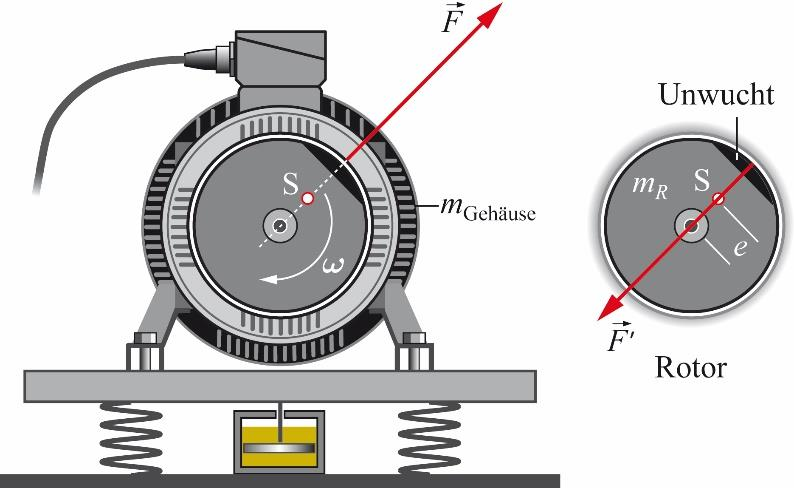
\includegraphics[height=3cm,center,keepaspectratio=true]{Images/unwuchterregung.png}
		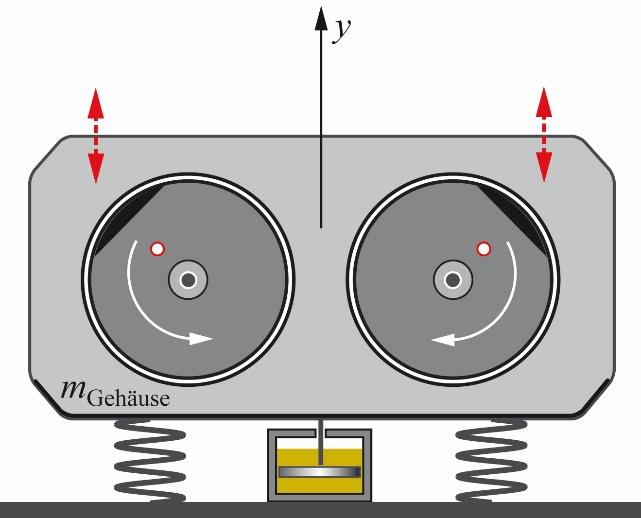
\includegraphics[height=3cm,center,keepaspectratio=true]{Images/unwuchterregung_doppelt.png}
	\end{minipage}
\end{center}

\begin{center}
	\begin{minipage}{0.28\textwidth}
		\unitText{$\omega$}{Kreisfrequenz der Störung}{$\frac{rad}{s}$} \\
		\unitText{$\omega_0$}{Kreisf. ungedämpfter Schwingung}{$\frac{rad}{s}$} \\
		\unitText{$\omega_r$}{Resonanzkreisfrequenz}{$\frac{rad}{s}$} \\
		\unitText{$\eta$}{dimensionslose Frequenz}{$1$} \\
		\unitText{$\varphi$}{Phase}{$rad$}
	\end{minipage}
	\begin{minipage}{0.2\textwidth}
		\unitText{$A$}{Amplitude}{$m$} \\
		\unitText{$A_r$}{Resonanzamplitude}{$m$} \\
		\unitText{$D$}{Dämpfungsgrad}{$1$} \\
		\unitText{$V$}{Vergrösserungsfunktion}{$?$}
	\end{minipage}
\end{center}



\subsubsection{Serienschwingkreis}
\formula{$L \ddot{I} + R_s \dot{I} + \dfrac{1}{C} I = \omega U_0 \sin(\omega t + \dfrac{\pi}{2})$}
\formula{$I_0 = \dfrac{\omega U_0}{L \sqrt{(\omega^2_0 - \omega^2)^2 + (2 D \omega_0 \omega)^2}}$}
\formula{$\varphi = \arctan \left( \dfrac{2 D \omega_0 \omega}{\omega^2_0 - \omega^2} \right) - \dfrac{\pi}{2}$}
\formula{$\omega_r = \omega_0$}
\formula{$I_{0r} = \dfrac{U_0}{R_s}$}
\formula{$V = \dfrac{\eta^2}{\sqrt{(1 - \eta^2)^2 + (2 D \eta)^2}}$}
\formula{$\varphi_U = \arctan \left( \dfrac{2 D \eta}{1 - \eta^2} \right) - \pi$}
\formula{$D = \dfrac{R_s}{2} \sqrt{\dfrac{C}{L}}$}

\subsubsection{Parallelschwingkreis}
\formula{$L \ddot{U} + R_s \dot{U} + \dfrac{1}{L} U = \omega I_0 \sin(\omega t + \dfrac{\pi}{2})$}
\formula{$U_0 = \dfrac{\omega I_0}{C \sqrt{(\omega^2_0 - \omega^2)^2 + (2 D \omega_0 \omega)^2}}$}
\formula{$\varphi = \arctan \left( \dfrac{2 D \omega_0 \omega}{\omega^2_0 - \omega^2} \right) - \dfrac{\pi}{2}$}
\formula{$\omega_r = \omega_0$}
\formula{$U_{0r} = R_p I_0$}
\formula{$V = \dfrac{1}{\sqrt{(1 - \eta^2)^2 + (2 D \eta)^2}}$}
\formula{$\varphi_I = \arctan \left( \dfrac{2 D \eta}{1 - \eta^2} \right)$}
\formula{$D = \dfrac{1}{2 R_p} \sqrt{\dfrac{L}{C}}$}










\section{Wellen}
\subsection{Wellengeschwindigkeit}

\begin{center}
	\begin{minipage}{0.4\textwidth}
		\unit{$u_L$}{Elastische Longitudinalwellen}{$\frac{m}{s}$}
	\end{minipage}%%% to prevent a space
	\begin{minipage}{0.2\textwidth}
		\formula{$u_L = \sqrt{\dfrac{E}{\varrho}}$}
	\end{minipage}
\end{center}
\begin{center}
	\begin{minipage}{0.4\textwidth}
		\unit{$u_T$}{Elastische Transversalwellen}{$\frac{m}{s}$}
	\end{minipage}%%% to prevent a space
	\begin{minipage}{0.2\textwidth}
		\formula{$u_T = \sqrt{\dfrac{G}{\varrho}}$}
	\end{minipage}
\end{center}
\begin{center}
	\begin{minipage}{0.4\textwidth}
		\unit{$u_T$}{Transversalwellen auf einem Seil oder einer Saite}{$\frac{m}{s}$}
	\end{minipage}%%% to prevent a space
	\begin{minipage}{0.2\textwidth}
		\formula{$u_T = \sqrt{\dfrac{F}{\varrho A}}$}
	\end{minipage}
\end{center}
\begin{center}
	\begin{minipage}{0.4\textwidth}
		\unit{$u_S$}{Schwerewellen in tiefem Wasser}{$\frac{m}{s}$}
	\end{minipage}%%% to prevent a space
	\begin{minipage}{0.2\textwidth}
		\formula{$u_S = \sqrt{\dfrac{g \lambda}{2 \pi}}$}
	\end{minipage}
\end{center}
\begin{center}
	\begin{minipage}{0.4\textwidth}
		\unit{$u_S$}{Schwerewellen in flachem Wasser}{$\frac{m}{s}$}
	\end{minipage}%%% to prevent a space
	\begin{minipage}{0.2\textwidth}
		\formula{$u_S = \sqrt{g h}$}
	\end{minipage}
\end{center}
\begin{center}
	\begin{minipage}{0.4\textwidth}
		\unit{$u_K$}{Kapillarwellen}{$\frac{m}{s}$}
	\end{minipage}%%% to prevent a space
	\begin{minipage}{0.2\textwidth}
		\formula{$u_K = \sqrt{\dfrac{2 \pi \sigma}{\varrho \lambda}}$}
	\end{minipage}
\end{center}
\begin{center}
	\begin{minipage}{0.3\textwidth}
		\unit{$u$}{Schallwellen in Fluiden}{$\frac{m}{s}$}
	\end{minipage}%%% to prevent a space
	\begin{minipage}{0.3\textwidth}
		\formula{$u = \sqrt{\dfrac{1}{\varrho \kappa}}$}
	\end{minipage}
\end{center}
\begin{center}
	\begin{minipage}{0.3\textwidth}
		\unit{$u_G$}{Schallwellen in Gasen}{$\frac{m}{s}$}
	\end{minipage}%%% to prevent a space
	\begin{minipage}{0.3\textwidth}
		\formula{$u_G = \sqrt{\dfrac{\varkappa p}{\varrho}}$}
		\formula{$u_G = \sqrt{\dfrac{\varkappa R T}{M}}$}
	\end{minipage}
\end{center}
\begin{center}
	\begin{minipage}{0.3\textwidth}
		\unit{$u_G$}{elektromagnetische Wellen}{$\frac{m}{s}$}
	\end{minipage}%%% to prevent a space
	\begin{minipage}{0.3\textwidth}
		\formula{$u = \dfrac{c}{n}$}
	\end{minipage}
\end{center}

\begin{center}
	\begin{minipage}{0.3\textwidth}
		\unit{$A$}{Fläche}{$m^2$} \\
		\unit{$E$}{Elastizitätsmodul}{$\frac{N}{m^2}$} \\
		\unit{$F$}{Spannkraft}{$N$} \\
		\unit{$G$}{Schubmodul}{$\frac{N}{m^2}$} \\
		\unit{$M$}{Molmasse}{$\frac{kg}{mol}$} \\
		\unit{$R$}{Universale Gas-Konstante (8.3145)}{$\frac{J}{K mol}$} \\
		\unit{$T$}{absolute Temperatur}{$K$} \\
		\unit{$c$}{Lichtgeschwindigkeit}{$\frac{m}{s}$} \\
		\unit{$g$}{Erdbeschleunigung}{$\frac{m}{m^s}$}
	\end{minipage}%%% to prevent a space
	\begin{minipage}{0.3\textwidth}
		\unit{$h$}{Wassertiefe}{$m$} \\
		\unit{$n$}{Brechungsindex}{$1$} \\
		\unit{$p$}{Druck}{$Pa$} \\
		\unit{$u$}{Wellengeschwindigkeit}{$\frac{m}{s}$} \\
		\unit{$\kappa$}{Kompressibilität}{$Pa$} \\
		\unit{$\varkappa$}{Adiabatenexponent}{$1$} \\
		\unit{$\lambda$}{Wellenlänge}{$m$} \\
		\unit{$\varrho$}{Dichte}{$\frac{kg}{m^3}$} \\
		\unit{$\sigma$}{Oberflächenspannung}{$\frac{N}{m}$}
	\end{minipage}
\end{center}

\begin{center}
	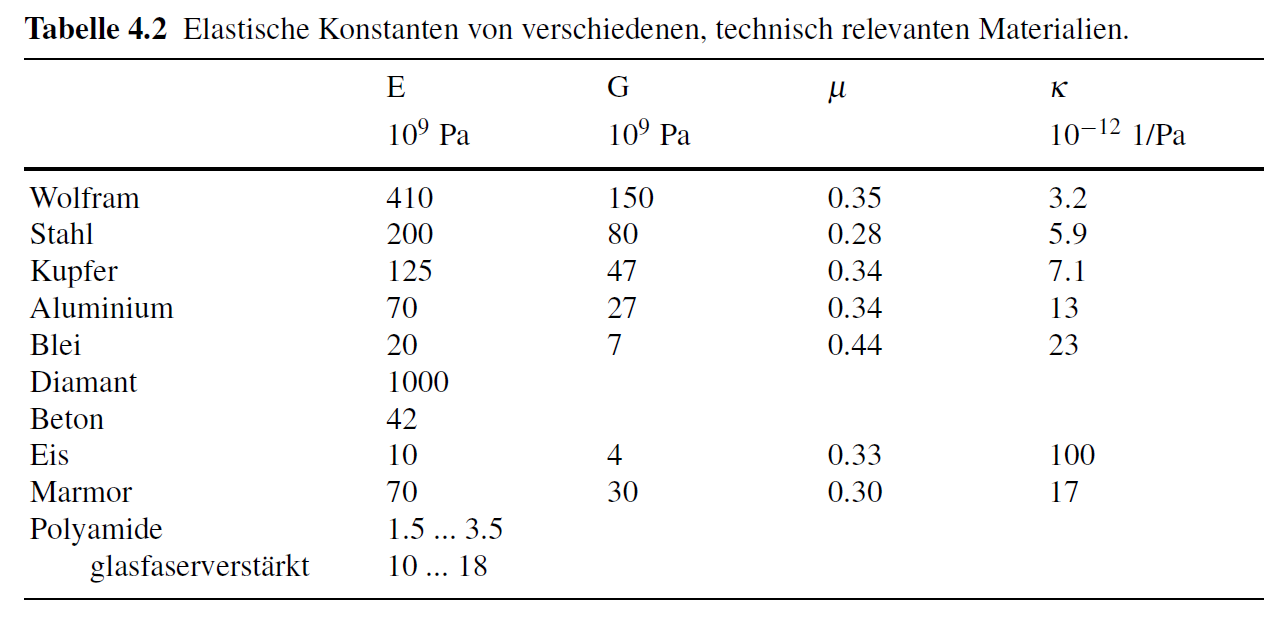
\includegraphics[height=5.5cm,keepaspectratio=true]{Images/elastische_konstanten.png}
\end{center}




\subsection{Harmonische Wellen}
\begin{center}
	\begin{minipage}{0.2\textwidth}
		\formula{$u = \dfrac{\omega}{k}$}
		\formula{$\lambda = \dfrac{2 \pi}{k} = \dfrac{u}{f}$}
		\formula{$\omega = \dfrac{2 \pi}{T}$}
	\end{minipage}%%% to prevent a space
	\begin{minipage}{0.3\textwidth}
		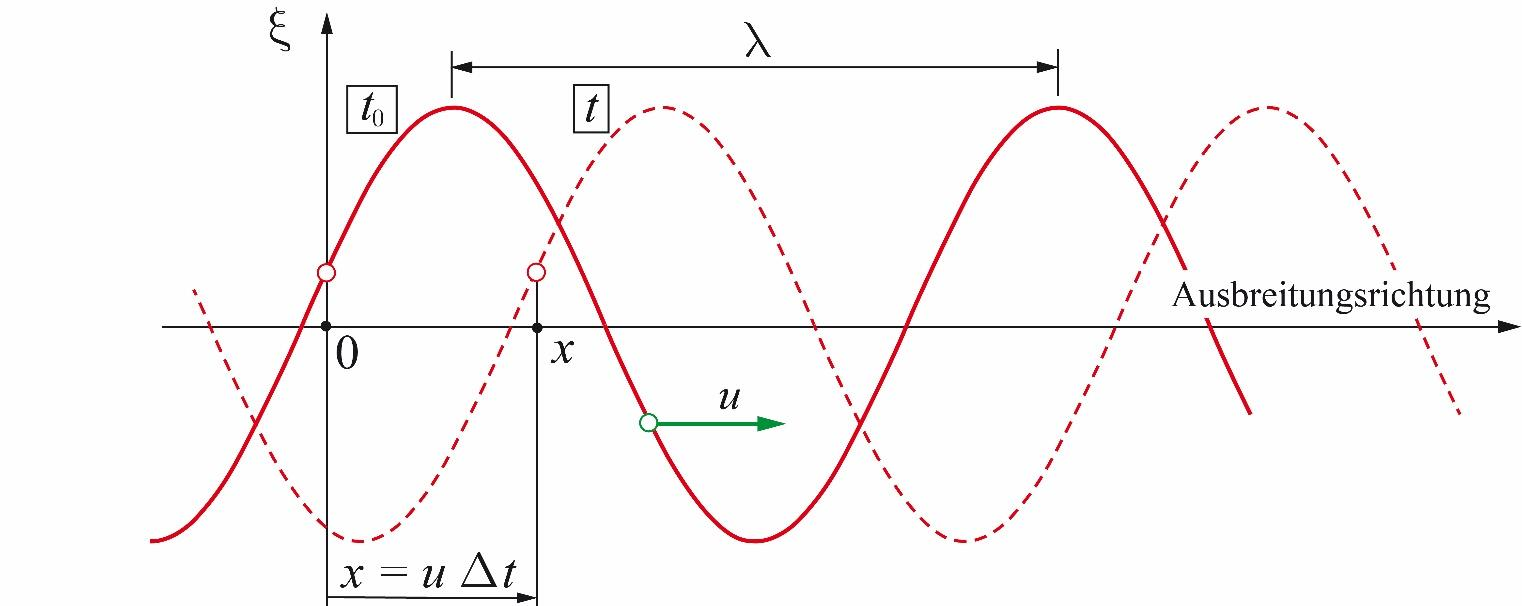
\includegraphics[height=3cm,keepaspectratio=true]{Images/harmonische_welle.png}
	\end{minipage}
\end{center}



























\subsubsection{Vorlage}

\begin{center}
	\begin{minipage}{0.3\textwidth}
		
	\end{minipage}%%% to prevent a space
	\begin{minipage}{0.3\textwidth}
		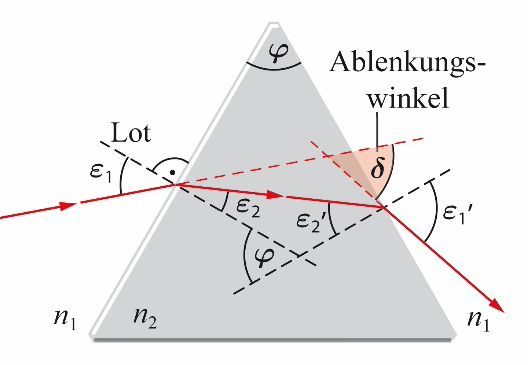
\includegraphics[height=3cm,keepaspectratio=true]{Images/prisma.png}
	\end{minipage}
\end{center}
	
\end{document}